\documentclass[12pt]{article}
\usepackage{a4}
\usepackage[english]{babel}
\setlength{\parindent}{0.35cm}
\pagestyle{headings}
\usepackage{graphicx}
%Multiple picture in one figure
%\usepackage{subfigure}
\usepackage{subfig}
\usepackage{listings}
\usepackage{color}
\usepackage{wrapfig}
%Floating-Umgebungen
\usepackage{float}
%Math-Environment
\usepackage{amsmath}
\usepackage{amssymb}
%Better SI-Units
\usepackage{siunitx}
%Using Appendix
\usepackage[title]{appendix}
%Using URL
\usepackage[hidelinks]{hyperref}
%Using Colored Tables
\usepackage{colortbl}
\newcommand{\gray}{\rowcolor[gray]{.90}}
\usepackage{esvect}
% Build fancy tables
\usepackage{booktabs}
%Configure geometry
\usepackage{geometry}
\geometry{
	a4paper,
	left=3cm,
	right=3cm,
	top=3cm,
	bottom = 3cm,
	}

\lstset{
	language=C++,
	basicstyle=\small\ttfamily,
	keywordstyle=\color{blue}\ttfamily,
	stringstyle=\color{red}\ttfamily,
	commentstyle=\color{green}\ttfamily,
	morecomment=[l][\color{magenta}]{\#},
}


\begin{document}
	
	\title{
		\textbf{\huge{CSE 446: Machine Learning Winter 2018 }} \\[2cm]
		\LARGE{Assignment 1}\\[1cm]
	}
	\author{from \\ Lukas Nies \\ University of Washington}
	\date{01/18/18}
	\clearpage\maketitle\thispagestyle{empty}
	\newpage

	\tableofcontents
	\setcounter{page}{0}
	\newpage
	
	% To start with section 1 labeled as section 0
	\setcounter{section}{-1}
	

\section{Policies}

\subsection{List of Collaborators}

\subsection{List of Acknowledgments}

\subsection{RTFM}

I have read and understood these policies.

\section{Problem: Criteria for Choosing a Feature to Split}

We build a tree with the dataset $D$ consisting $n$ negative examples (label 0) and $p$ positive examples (label 1). 

\subsection{Not Splitting}

If we are at the bottom of our decision tree and don't have any features left to split, consider the subset $D'$ of data $D$ with $n'$ negative and $p'$ positive examples. The smallest number of mistakes we can make in this subset is given by

\begin{align}
	\text{err}(D') = \min(n',p') = 
	\begin{cases}
		p' & \text{if } p'< n' \\
		n' & \text{if } n'< p'
	\end{cases}
\end{align}

The node itself is labeled accordingly, with $0$ if $n'< p'$ or with $1$ if $n'> p'$. 

\subsection{Splitting}

Now we have a new feature $\Phi$ which splits the subsection $D'$ according to the contingency table:
% Table generated by Excel2LaTeX from sheet 'Sheet1'
\begin{table}[htbp]
	\centering
	\caption{Add caption}
	\begin{tabular}{|c|c|c|}
		\toprule
		y     & \multicolumn{2}{c|}{phi} \\
		& \multicolumn{1}{c}{0} & 1 \\
		\cmidrule{2-3}    0     & $n_0$    & $n_1$ \\
		\cmidrule{2-3}    1     & $p_0$    & $p_1$ \\
		\bottomrule
	\end{tabular}%
	\label{tab:addlabel}%
\end{table}%
By splitting we generate two new sub-nodes: $(n_0,p_0)$ and $(n_1,p_1)$. The error for splitting is given by the sum of the errors of both nodes
\begin{align}
\text{err}(D') = \min(n_0,p_0) + \min(n_1,p_1),
\end{align}
where $n'=n_0 + n_1$ and $p'=n_1+p_1$. The error reduction rate ($\text{err}\_\text{red}$) is given by the reduction of error if comparing the error of "not splitting" with the error of "splitting", divided by the total number of examples in node $D'$:
\begin{align}
\text{\text{err}\_\text{red}}(D'): \frac{\min(n',p')-\left(\min(n_0,p_0) + \min(n_1,p_1)\right)}{\lvert D' \rvert}.
\end{align} 
Consider the maximal possible error (in this case for binary data) when $n'=p'=0.5 \lvert D' \rvert$
\begin{align}
\text{err}_\text{max}(D')=\min(n',p')=0.5\lvert D' \rvert,
\end{align}
then the maximal possible error reduction is given by 
\begin{align}
\text{\text{err}\_\text{red}}(D'): \frac{\min(0.5 \lvert D',0.5 \lvert D')-\left(\min(n_0,p_0) + \min(n_1,p_1)\right)}{\lvert D' \rvert} = 0.5,
\end{align}
where either $p_0=0$ or $n_0=0$ and $p_1=0$ or $n_1=0$ (maximal information gain).

\subsection{Mutual Information}

\begin{figure}[b!]
	\centering
	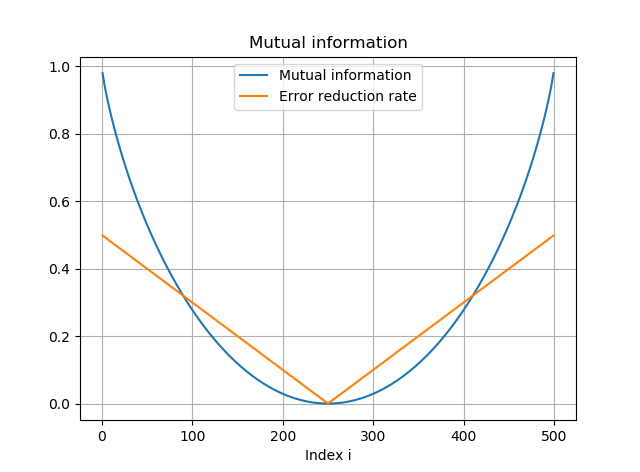
\includegraphics[width=0.65\linewidth]{../Problem_1/Figure_1.png}
	\caption{Comparison of mutual information between feature and label and error reduction rate for splitting the dataset.}
	\label{fig:1.3}
\end{figure}

The mutual information is a measure of information gain when splitting a dataset. In figure \ref{fig:1.3} the mutual information and the error reduction rate are plotted for problem $1.3$. 








%\chapter*{Bibliography}
%\addcontentsline{toc}{chapter}{Bibliography}%	

\bibliographystyle{unsrt}
\bibliography{./bib}





\end{document}  